% !TEX root = ../AiiDA_tutorial.tex

\section{\label{sec:workchain_demonstration}WorkChains, a real-world example: computing a band structure for a simple crystal structure}

\textbf{Note}: \emph{If you still have enough time, you might want to check first Appendix~\ref{sec:convpressure} before continuing with this section.}

As a final demonstration of the power of WorkChains in AiiDA, we want to give a demonstration of a WorkChain that we have written that will take a structure as its only input and will compute its band structure.
All of the steps that would normally have to be done manually by the researcher, choosing appropriate pseudopotentials, energy cutoffs, k-points meshes, high-symmetry k-point paths and performing the various calculation steps, are performed automatically by the WorkChain.

The demonstration of the workchain will be performed in a Jupyter notebook.
To run it, follow the instructions that were given for the querybuilder notebook in section \ref{sec:querybuilder}.
The only difference is that instead of selecting the notebook in the \texttt{querybuilder} directory, go to \texttt{pw/bandstructure} instead and choose the \texttt{bandstructure.ipynb} notebook.
There you will find some example structures that are loaded from COD, through the importer integrated within AiiDA.
Note that the required time to calculate the bandstructure for these example structures ranges from 3 minutes to almost half an hour, given that the virtual machine is running on a single core with minimal computational power.
It is not necessary to run these examples as it may take too long to complete.
For reference, the expected output band structures are plotted in Fig.\,\ref{fig:workchain_band_structures}.

\begin{figure}
\begin{subfigure}{.5\textwidth}
  \centering
  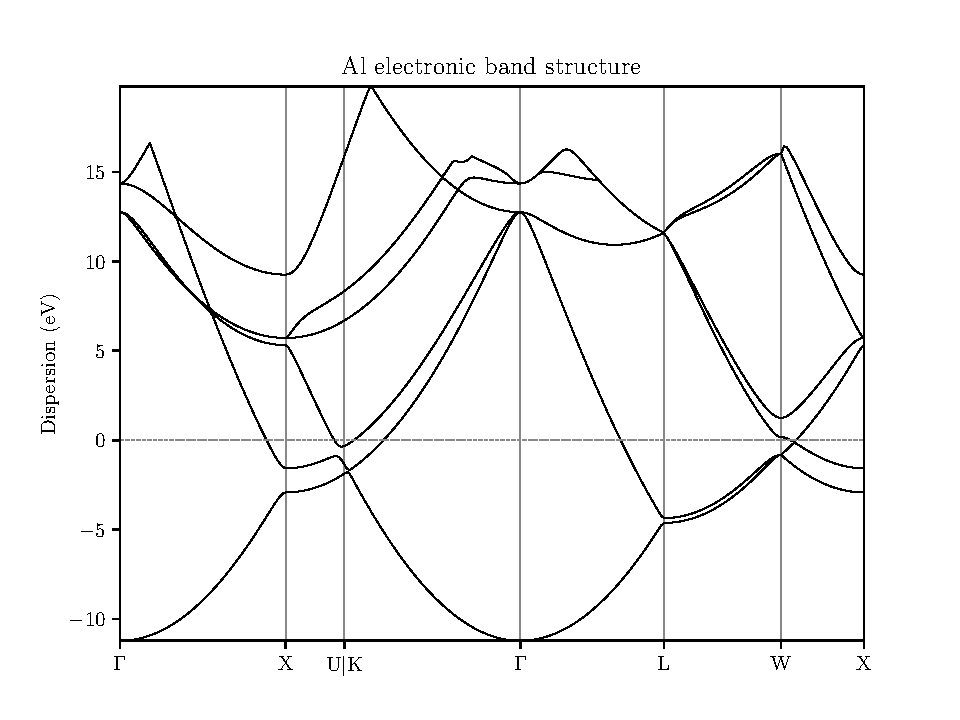
\includegraphics[width=.9\linewidth]{sections/images/bandstructures/Al_bands.pdf}
  \caption{Al}
  \label{fig:workchain_band_structures_Al}
\end{subfigure}%
\begin{subfigure}{.5\textwidth}
  \centering
  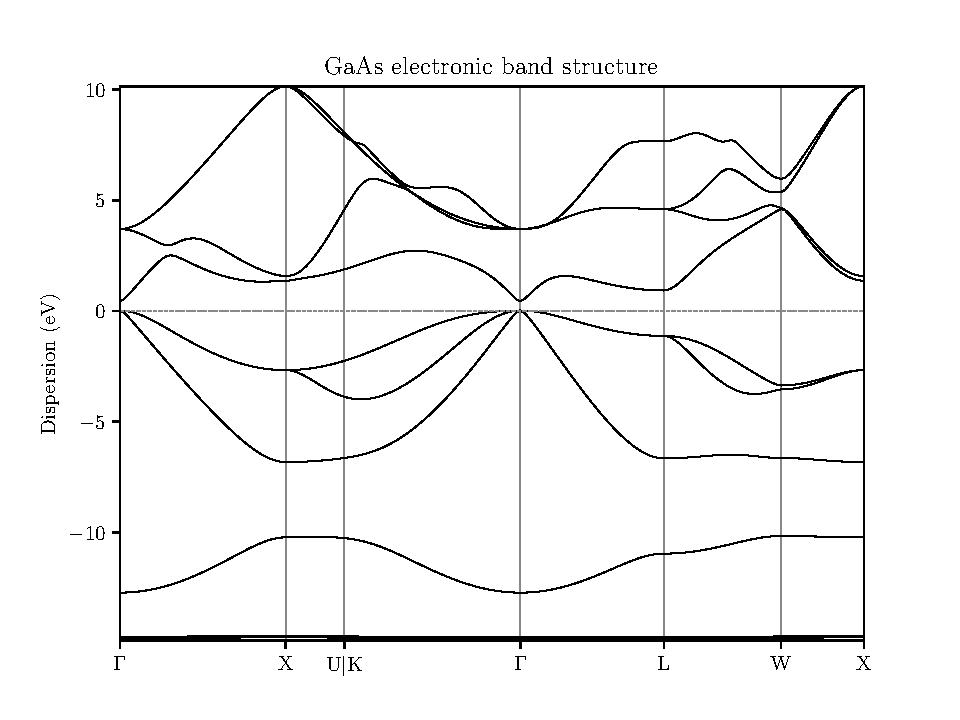
\includegraphics[width=.9\linewidth]{sections/images/bandstructures/GaAs_bands.pdf}
  \caption{GaAs}
  \label{fig:workchain_band_structures_GaAs}
\end{subfigure}%
\newline
\begin{subfigure}{.5\textwidth}
  \centering
  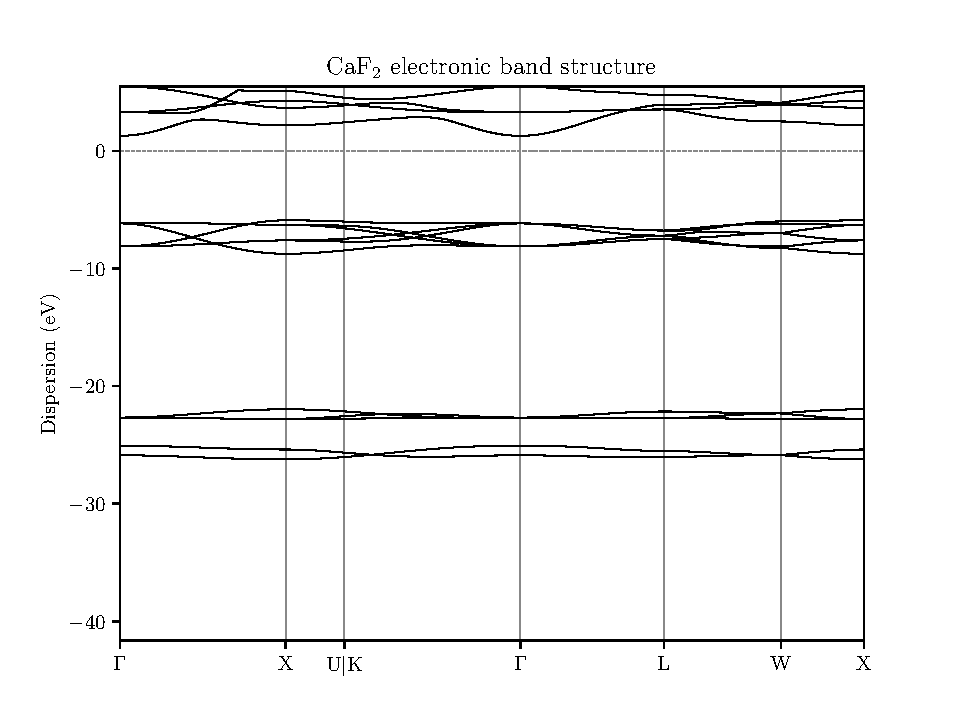
\includegraphics[width=.9\linewidth]{sections/images/bandstructures/CaF2_bands.pdf}
  \caption{CaF$_2$}
  \label{fig:workchain_band_structures_CaF2}
\end{subfigure}%
\begin{subfigure}{.5\textwidth}
  \centering
  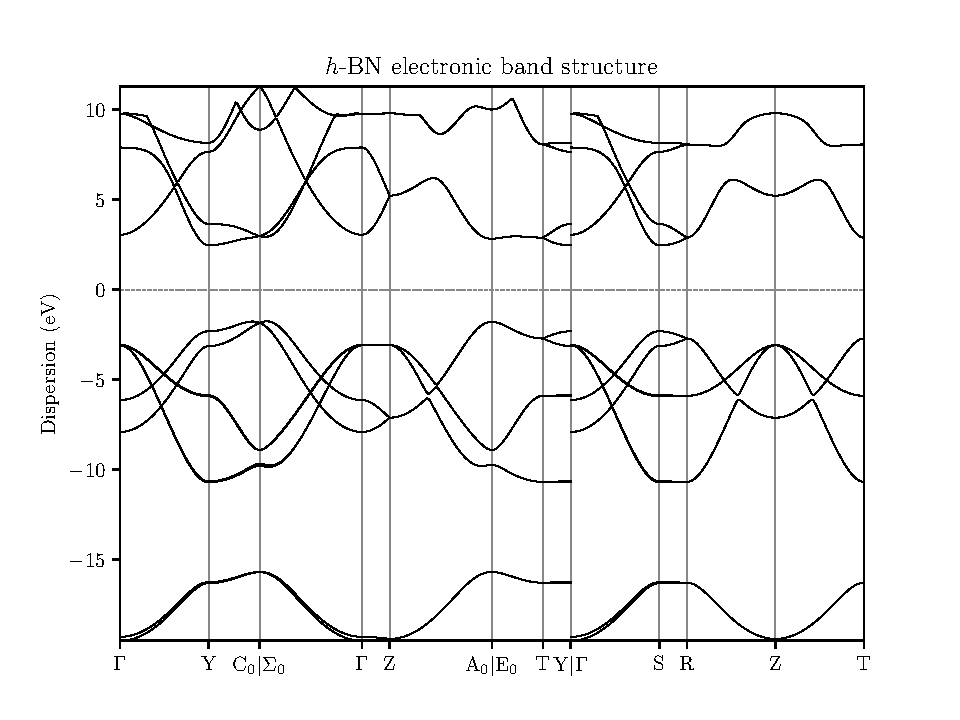
\includegraphics[width=.9\linewidth]{sections/images/bandstructures/hBN_bands.pdf}
  \caption{$h$-BN}
  \label{fig:workchain_band_structures_hBN}
\end{subfigure}%
\caption{Electronic band structures of four different crystal structures computed with AiiDA's PwBandsWorkChain}
\label{fig:workchain_band_structures}
\end{figure}
